\chapter{Implementation}
\label{implementation}
We present a computer program which takes in textual phrases in English, determines all oronyms for that phrase and then visualizes them with associated information to indicate the likelihood of interpretation.
To accomplish this, the program has three major functional parts: a custom phonetic dictionary, a command-line oronym generator, and a OpenGL oronym-parse-tree visualization generator.

\section{Customized Phonetic Dictionary} 
\label{section:Implementation:customizedPhoneticDictionary}

In order to discover oronyms for each phrase, we first needed to determine how each phrase is pronounced.  Pronunciation can vary depending on the speakers accent, so it was important for us to (1) chose an accent that we could easily replicate and (2) find a dictionary that supported that accent.  

We decided to utilize a General American accent, due to its ubiquity in media and news sources. The General American accent, also known as the ``Standard American English" dialect, is not spoken by the majority of people in America, but is used as an ``average accent".  It most closely resembles the Midwestern accent using in the area in Figure ~\ref{fig:generalAmericanMap} and more commonly recognized as ``the newscaster accent". Newscasters learn this accent for national TV, because it is the ``least-accented" of the American accents.  

\begin{center}
\begin{figure}
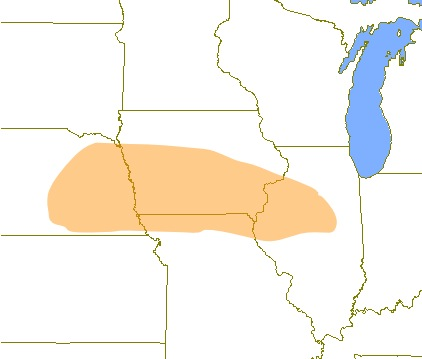
\includegraphics[width=60mm]{General_American.jpg}
\captionfonts
\caption[Geographic Origin of General American]{This is the geographic area whose accent most closely resembles the General American Accent \cite{generalAmericanAccentMap} }
\label{fig:generalAmericanMap}
\end{figure}
\end{center}

\subsection{Dictionary Options}
\label{subsection:dictionaryOptions}

We considered using three different phonetic dictionaries: the CMU dictionary, LC-STAR dictionary and UNISYN dictionary\cite{lcStarWebsite} \cite{cmuDictWebsite}  \cite{unisynLexiconWebsite}.  We started out by looking at the LC-STAR dictionary, but quickly decided that it wasn’t going to be as useful to us, because the LC-Star project is relatively focused on Speech-to-Speech or Text-to-Speech tech. In addition, the dictionary is not well-maintained.  

The CMU dictionary showed promise, but had a few shortcomings.  It had a very simple way of encoding words:  first the word, then the identifier number in parens (if needed), then a space, then a one-to-two char code for each sound in the word, with the numbers 0, 1, 2 appended to indicate emphasis (if needed), separated by spaces.  An example of a CMU dictionary entry can be seen in Figure ~\ref{fig:CMUdictAbbreviate}.

\begin{figure}
\begin{center}
\begin{verbatim}
ABBREVIATE  AH0 B R IY1 V IY0 EY2 T
\end{verbatim}
\captionfonts
\caption[CMU dictionary entry example]{Here is the CMU dictionary entry for the word ``abbreviate" }
\label{fig:CMUdictAbbreviate}
\end{center}
\end{figure}

The problem that arose with this format, was that there was no explicit definition of where to hyphenate the word when splitting it up.  This causes problems for words in song lyrics, where each note has its own syllable underneath it, and each syllable might have many different sounds. 
The benefits of the CMU dictionary over some other dictionaries were that (1) it was actively maintained, (2) it included proper nouns, which are often found in lyrics, but not in dictionaries, and (3) it was ridiculously easy to read.

The downsides were that (1) it included no part of speech data or hyphenation data, and (2) it used non-standard symbols for its phonetic alphabet.  
With the downsides and benefits in mind, the CMU dictionary could not be used in isolation, especially if we someday want to attempt generation of original lyrics (which part of speech data would be vital for).  

The UNISYN dictionary is used primarily to phonetically translate words into multiple accents.  It has its own formated dictionary, with a bunch of wildcards in it.  They also provide some semi-functioning perl scripts that allow you to specify a dialect you’d like to use (For example, a Californian would say “cooking” differently than someone from the Deep South, and both would say it differently than someone from London.  However, they are all speaking English.  The UNISYN dictionary facilitates this translation).  

It had all the information we needed, and then some.  However, it was case-insensitve, meaning that it didn't make it easy to differenciate pronunciations for some words. For example, the word ``nice" is pronounced differently from the city ``Nice", but they were both stored as ``nice" in the orthography of UNISYN.  The CMU dictionary did keep track of capitalization.  The obvious conclusion, then, was to grab the capitalizations from the CMU dictionary and put them in the UNISYN dictionary, aligning them by pronunciation and part of speech. 

However, we ran into a setback, mentioned in the very first article we found references to both dictionaries in:  the dictionaries were inconsistent\cite{polyakova_fusion_2007}.  They didn’t always put stresses in the same place, nor did they always have the same pronunciation.  Because of this, it was difficult to match words, especially words that were homographic heteronyms (same writing, different sounds, like ``Do you know what a buck \emph{does} to \emph{does}?").  Because of this, we decided to use the UNISYN dictionary exclusively.

\subsection{Custom dictionary fields}
\label{subsection:customDictionaryFields}

Here is the format for the fields in an entry in our custom phonetic dictionary, after we were done with fixing the UNISYN output:
\begin{center}
\textcolor{Aquamarine}{$<$\textbf{ortho}$>$} :
\textcolor{BurntOrange}{$<$\textbf{uniqueID}$>$} :
\textcolor{RoyalBlue}{$<$\textbf{partOfSpeech}$>$} :
\textcolor{Red}{$<$\textbf{SAMPAspelling}$>$} :
\textcolor{Rhodamine}{$<$\textbf{SAMPAnoEmph}$>$} :
\textcolor{Periwinkle}{$<$\textbf{extendedOrtho}$>$} :
\textcolor{Blue}{$<$\textbf{freq}$>$}
\end{center}

\begin{figure}
Example:
\begin{center}
{\tt 
\textcolor{Aquamarine}{transfer} :
\textcolor{BurntOrange}{2} :
\textcolor{RoyalBlue}{VB/VBP} :
\textcolor{Red}{tr\{ns"f3`r} :
\textcolor{Rhodamine}{tr\{nsf3`r} :
\textcolor{Periwinkle}{\{trans==fer\}} :
\textcolor{Blue}{7184}
}
\captionfonts
\caption[Custom dictionary entry example]{Here is an example an entry in our custom phonetic dictionary, using the word ``transfer" }
\label{fig:customDictionaryEntryExample}
\end{center}
\end{figure}

\textcolor{Aquamarine}{$<$\textbf{ortho}$>$} is the regular spelling of the word

\textcolor{BurntOrange}{$<$\textbf{uniqueID}$>$} is a number (and optional string) used to differentiate homographs.

\textcolor{RoyalBlue}{$<$\textbf{partOfSpeech}$>$} is used to identify the specific part of speech

\textcolor{Red}{$<$\textbf{SAMPAspelling}$>$} is the breakdown of the word, phonetically. It uses the SAMPA alphabet, and separators to show where breaks in the word are, and how they’re emphasized. If a separator is ' \$ ', the following phones (until the next separator) are not emphasized.  If it's ' \% ', then they are the secondary emphasis.  If it's ' `` ', then they are the primary emphasis.

\textcolor{Rhodamine}{$<$\textbf{SAMPAnoEmph}$>$} is the same as \emph{<SAMPASpelling>}, but with all emphasis characters stripped out.  We chose to add this field so that we could more-easily look up phonetic sequence matches. 

\textcolor{Periwinkle}{$<$\textbf{extendedOrtho}$>$} allows for stemming analysis of words, for possible use in future work.

\textcolor{Blue}{$<$\textbf{freq}$>$} is the frequency at which the word occurs in language, according to UNISYN. The frequency count is ``taken from a composite of a number of on-line sources of word-frequency. It includes frequencies from the British National Corpus and Maptask, and frequencies derived from Time articles and on-line texts such as Gutenberg. They were weighted to give more importance to sources of spoken speech, and also to increase the numeric frequency of smaller corpuses"\cite{fitt_documentation_2000}.


An example of a entry in our custom phonetic dictionary can be seen in \textbf{Figure ~\ref{fig:customDictionaryEntryExample} }.
\subsection{Transferring the dictionary to a sqlite database}
\label{subsection:transferringTheDictionaryToASqliteDatabase}

Because there are several hundred thousand entries in our phonetic dictionary, it was necessary to have a database, rather than store them all in-program in a multi-dimensional array.  We decided to use a SQLite database for this purpose.  

To turn the colon-delimited dictionary file into a SQLite database, we decided to use a program called the “SQLite Database Browser”, an open source, public domain, freeware visual tool to create, design, and edit SQLite3.x database files.  We specifically used version 2.0b1 of the program, which was built with version 3.6.18 of the SQLite engine\cite{sqliteDatabaseBrowser}.

\section{Oronym Generation}
\label{oronymGeneration}

\subsection{Step 1: Find all phonemic variations of an orthographic phrase}
\label{subsection:stepOneFindAllSAMPAphrase}

First, our program takes an orthographic phrase to find oronyms for.

\begin{figure}[h]
\begin{center}
\begin{tabular}{|c|}
\hline
`a nice cold hour' \\
\hline
\end{tabular}
\label{fig:oronymGeneration:orthoPhraseInput}
\end{center}
\end{figure}

We then tokenize this phrase into its component words, using whitespaces as a delimiter. 
\begin{figure}[h]
\begin{center}
\begin{tabular}{|c|}
\hline
`a', `nice', `cold', `hour' \\
\hline
\end{tabular}
\label{fig:oronymGeneration:tokenizedInputOrthoPhraseWords}
\end{center}
\end{figure}


For each word in the phrase, we query our phonetic dictionary for all possible SAMPA pronunciations.

\begin{figure}[h]
\begin{center}
\begin{tabular}{|c|}

\hline
`a' \rightarrow  \tt{e}, \tt{@}, \tt{A} \\

`nice' \rightarrow   \tt{naIs}, \tt{nis} \\

`cold' \rightarrow \tt{kould} \\

`hour' \rightarrow \tt{aU\char18 r} \\
\hline
\end{tabular}
\captionfonts
\caption[queryDBwithOrthoWordForSampa example]{ In this and all subsequent diagrams, a `string in quotes' indicates an orthographic word or phrase, and a \texttt{monospaced string} indicates that it is a SAMPA word or phrase.  }
\label{fig:oronymGeneration:queryDBwithOrthoWordForSampa}
\end{center}
\end{figure}

Now that we have the pronunciation of each of the words in the form of SAMPA strings, we can list all the possible phonetic permutations of the original phrase.

\begin{figure}[h]
\begin{center}
\begin{tabular}{|c|}

\hline
e naIs kould aU\char18 r \\

@ naIs kould aU\char18 r \\

A naIs kould aU\char18 r  \\

e nis kould aU\char18 r \\

@ nis kould aU\char18 r \\

A nis kould aU\char18 r \\
\hline
\end{tabular}
\captionfonts
\caption{}
\label{fig:oronymGeneration:orthoWordPhoneticPermutations}
\end{center}
\end{figure}


The pseudocode for this process can be reviewed in figure ~\ref{fig:psuedoCode:findAllPhoneSeqsForOrthoPhrase}.

\setlength\LTleft{-2in}
\begin{figure}
\begin{verbatim}
findAllPhoneSeqsForOrthoPhrase( orthoPhrase ) {
  allFullPhrasePhoneSeqs = empty list of list of phones
  orthoWords = split orthoPhrase on spaces
  
  origNumFullPhrases = 0
  for( orthoWord in orthoWords with index i ) {
    nextWordSampaPhoneSeqs = possible phone seqs following orthoWord
    
    if ( orthoWord is the first word in orthoPhrase ) {
      for( phoneSubSeq in nextWordSampaPhoneSeqs ) {
        append phoneSubSeq to allFullPhrasePhoneSeqs[i]
      }
    } else {
      origNumFullPhrases = allFullPhrasePhoneSeqs.size()
      if there’s more than one vector <phone> in nextWordSampaPhoneSeqs
        then we need to create duplicates of all existing allFullPhrasePhoneSeqs
    }
    
    for( m = 0 to allPhrasePhoneSeqs.size() ) {
      phraseToAppendIndex = m / origNumFullPhrases
      phoneSeqToAppend = nextWordSampaPhoneSeqs[phraseToAppendIndex]
      append phoneSeqToAppend to allFullPhrasePhoneSeqs[m]
    }
  }

  return allFullPhrasePhoneSeqs
}
\end{verbatim}
\captionfonts
\caption[Pseudocode for findAllPhoneSeqsForOrthoPhrase]{ Algorithm to get all phonetic sequences for an orthographic phrase. }
\label{fig:psuedoCode:findAllPhoneSeqsForOrthoPhrase}
\end{figure}
%\setlength\LTleft{2in}



\subsection{Step 2: Finding all Orthographic phrases for a Phonemic Sequence}
\label{subsection:stepTwoFindOrthoforSAMPA}

Then, for each phonemic phrase, we want to figure out all valid orthogrpahic interpretations.  For this, we have to go back to our phonetic dictionary.

The ideal way to think about searching for words in a phonetic sequence is by picturing the phoenetic sequence in a tree form.  For example, if I had a phonetic tree with the entire dictionary in it, each phonetic tree node would have at least 45 child nodes: one for each phone.  A node might also have ``word" nodes, if the phones along the path to that node construct a valid orthographic word:

When there are multiple orthographic interpretations at a single phonetic node, the most likely interpretation can be determined by checking the frequency of use for each word.  For example, the sequence ``n aI s" is much more likely to be ``nice" than ``gneiss".  Figure ~\ref{fig:wordTree} shows a visual representation of traversing an entire dictionary's phonetic tree for nodes along the paths for the SAMPA sequences `aIs' and `nice'.

\begin{figure}[h]
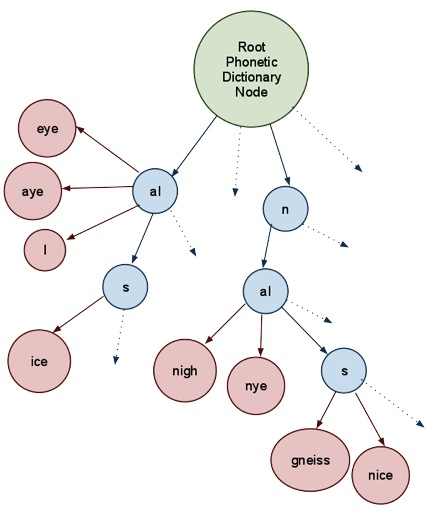
\includegraphics[width=90mm]{wordTree.jpg}
\captionfonts
\caption{}
\label{fig:wordTree}
\end{figure}

We can use this dictionary tree method to discover valid orthographic interpretations for each phonetic sequence.  Using the dictionary tree method above, we can orthographically interpret each phonetic transcription of our root orthographic phrase, as shown in figure ~\ref{fig:aNiceColdHourPhoneToOrthoGraph}:



\begin{figure}[h]
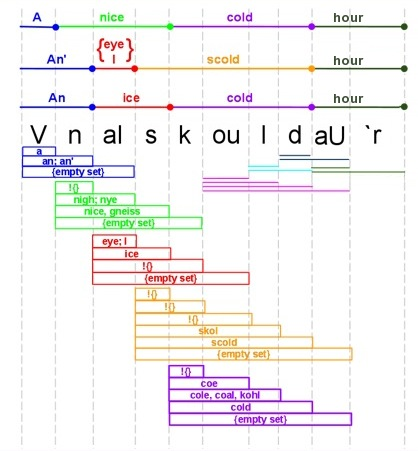
\includegraphics{aNiceColdHourPhoneToOrthoBreakdown.jpg}
\captionfonts
\caption{}
\label{fig:aNiceColdHourPhoneToOrthoGraph}
\end{figure}

Once we have grabbed all the orthographic interpretations for each phonetic sequence, we combine them all into a orthographic oronym phrase list. This process may leave us with some redundant oronyms, so we de-duplicate that list.

This process gives us a list of all unique and valid oronyms for the original root phrase.

In the case of ``a nice cold hour", this returns 290 oronyms, as seen in the first column of figure ~\ref{table:aNiceColdHourOronymWithFreqsTable}.



The pseudocode for this process can be reviewed in figure ~\ref{fig:psuedoCode:discoverOronymsForPhrase}
\setlength\LTleft{-2in}
\begin{figure}
\begin{verbatim}
discoverOronymsForPhrase( origOrthoPhrase, includeDeadends ) {
   orthoMisheardAsPhrases = empty list
   allPhoneSeqsOfOrigPhrase = origOrthoPhrase.findAllPhoneSeqs()
   
   for( curPhoneSeqWithEmph in allPhoneSeqsOfOrigPhrase ) {
      // Remove emphasis marking for easier lookups
      curPhoneSeq = curPhoneSeqWithEmph.stripEmphasis()

      altOrthoPhrases = findOrthoStrsForPhoneSeq( curPhoneSeq )
      
      for( altOrthoPhrase in altOrthoPhrases ) {
         // Ensure it contains valid ortho text in all cases, and if
         // includeDeadends=false, contains no deadEndDelims so we only add
         // fully valid strings
         if ( ( includeDeadends == true &&
                altOrthoPhrase != deadEndDelim1 &&
                altOrthoPhrase != deadEndDelim2 ) ||
              ( altOrthoPhrase.contains( deadEndDelim1 ) == false &&
                altOrthoPhrase.contains( deadEndDelim2 ) == false ) ) {
            append altOrthoPhrase to orthoMisheardAsPhrases
         }
      }
   }
   
   orthoMisheardAsPhrases.removeDuplicates()

   return orthoMisheardAsPhrases
}
\end{verbatim}
\captionfonts
\caption[Pseudocode for discoverOronymsForPhrase]{ Algorithm to get all oronyms for an orthographic phrase. }
\label{fig:psuedoCode:discoverOronymsForPhrase}
\end{figure}
\setlength\LTleft{2in}




\subsection{Word Frequency Evaluation}
\label{subsection:wordFrequencyEvaluation}

Next, we want to evaluate all our oronyms based on how common each oronym's component words are.  For example, ``a nice cold hour" is much more likely to be heard ``a gneiss cold hour", even though both are phonetically identical.

To do this, we tokenize each oronym phrase into its component words, once again using non-newline whitespaces as a delimiter. 

Then, we query our phonetic dictionary with each word for the word's frequency value.  We store each word's value separately. When we have retrieved the frequencies for all the words in a phrase, we then add all the frequencies up to give a combined-frequency of the entire phrase.

You can see these frequency counts for the phrase ``a nice cold hour" in figure ~\ref{table:aNiceColdHourOronymWithFreqsTable}.




\section{Visual Representation}
\label{section:implementation:visualRepresentation}

We go about building the visual representation of the oronym parse tree in much the same way that we build the textual list of oronyms, with one important difference: our oronym parse trees may contain oronym fragments.   To deal with these we've got to keep track of all our abandoned sub-phrases.

Our algorithm for doing this is recursive, called from a parent function that draws the tree's `seed' sphere. This parent function is documented in figure ~\ref{fig:psuedoCode:buildAndDrawFullTree}


We start in the parent function by getting all the oronyms of our orthographic phrase, using the process in sections  ~\ref{subsection:stepOneFindAllSAMPAphrase} ~\ref{subsection:stepTwoFindOrthoforSAMPA}.  However, instead of ignoring any incomplete orthographic interpretation of a phonetic sequence, as we do in section~\ref{subsection:stepTwoFindOrthoforSAMPA}, we add them to the list of oronyms, keeping track of them by appending `xxx' or `fff' to the end of the incomplete  oronym string.  Then, we tokenize our phrases by whitespace, and look up the frequency of each word, keeping track of only the maximum and minumum values.  We will later scale our branches' radiuses using these values.

Once we have all the partial and complete oronyms and the max and min word frequency values for them, we pass them into our recursive function, along with the radius of the seed sphere.  That radius will be the beginning radius of each first-level branch.  

Inside our recursive function, we pull the first word out of every orthographic phrases we were passed, and create a set of unique first words.  

We then go through this set of unique first words iteratively.

For each word, we look up frequency in the phonetic dictionary.  Then, we use the max and min frequencies that we found in our parent function, plus constants for max and min radius size, to scale that frequency into a usable radius size. 

Then, we check the contents of the word. 

If the word is ``xxx" or ``fff", then it's not a word at all--just an indication of the dead end of a partial oronym.  In this case, we draw a red sphere with the radius of the branch's ancestor, using the parameter past into our recursive function for `lastRadius'.  

If the word is ``\_\_\_SUCCESS!\_\_\_", that is also not a real word. It indicates that a full oronym has been successfully found, and is terminating at that point. This time, we draw a green sphere using the `lastRadius' parameter for size.

If the word is neither of these, then it must be a real word.  We then draw a cylinder ``branch" representing that word. The cylinder's bottom radius is equal to \emph{lastRadius}, and the top radius is equal to the scaled radius that we got from the word's frequency.  

After we draw the cylinder, we then go through the full list of phrases, and compile a list of all phrases that start with the word we just drew the cylinder for.  Then, we remove the first word from each of those phrases, deduplicating the resulting list of ``tail" phrases.

Then, we change our material color (so that different levels of branches will be different colors), and make a recursive call to our current function, passing as parameters the scaled radius and the list of tail phrase.

After this recursive call, we change our color material back to whatever it was before the call, and then continue on to the next unique first word in our set.


Once we have looped through all our unique first words, we know we're done drawing that set of branches, and we return.  

This gives us the oronym parse tree seen in figure ~\ref{fig:treeEmptyTillIsSad}.  As shown in figure ~\ref{fig:treeEmptyTillIsSadAnnotated} (the annotated version of figure ~\ref{fig:treeEmptyTillIsSad}) each branch on the tree represents a single orthographic word.


\begin{figure}
\begin{verbatim}
buildAndDrawFullTree( orthoPhrase ) {
   fullPhrases = orthoPhrase.discoverOronyms()
   (maxWordFreq, minWordFreq) = fullPhrases.getMaxAndMin()
   
   // Draw the tree's seed.
   glPushMatrix()
   {
      glTranslated(0.0, -1.0 * DEFAULT_BRANCH_LEN, 0.0)
      materials(GreenShiny)
      drawSphere(DEFAULT_RADIUS)
      materials(allMaterials.at( mat % allMaterials.size() ) )
      
      drawBranchesAtFork ( fullPhrases, DEFAULT_RADIUS )
   }
   glPopMatrix()
}
\end{verbatim}
\captionfonts
\caption[Code for buildAndDrawFullTree]{ Given an orthographic phrase, this function prepares to draw the tree }
\label{fig:psuedoCode:buildAndDrawFullTree}
\end{figure}


\begin{figure}
\begin{adjustwidth}{-1in}{}
\begin{verbatim}
drawBranchesAtFork( fullPhrases, lastRadius) {
   if( fullPhrases.size() == 0 ) {
      return
   }
   
   // Use a set to ensure no duplicates.
   firstWords = empty set
   
   for( phrase in fullPhrases ) {
      if( phrase.size() > 0 ) {
         firstWords.insert( phrase.firstWord() )
      }
   }
   
   // Calculate positioning variables for the spread of branches for firstWords.
   for ( curFirstWord in firstWords ) {
      firstWordFreq = curFirstWord.frequency()
      newAdditiveRadius = firstWordFreq.scaleToRadius()

      glPushMatrix()
      {
         // Translate and rotate into place
         if( curFirstWord == deadEndDelim1 || curFirstWord == deadEndDelim2 ) {
            // Draw a red sphere at the end of the last branch
         } else if ( curFirstWord == successDelim ) {
            // Draw a green sphere at the end of the last branch
         } else {
            // Draw a branch
            drawBranch( radiansToDegrees(tiltAngle), curXOffset, curYOffset,
                        newAdditiveRadius, lastRadius )
            
            // Find all phrases in fullPhrases that start with that firstWord
            tailsVect = fullPhrases.findAllWithPrefix(curFirstWord)
            
            // Change the colors for each branch level

            // Pass those phrases to drawBranchesAtFork
            drawBranchesAtFork( tailsVect, newAdditiveRadius, curXOffset, curYOffset )
            
            // Change the colors back to ensure consistency for each branch level
         }
      }
      glPopMatrix()
   }
}
\end{verbatim}
\end{adjustwidth}
\captionfonts
\caption[Code for drawBranchesAtFork]{ This is the function that facilitates the in-time drawing of the tree as we parse though our oronyms possibilities }
\label{fig:psuedoCode:drawBranchesAtFork}
\end{figure}

At the end of this process, we have generated a tree like the one in figure ~\ref{fig:treeEmptyTillIsSad}.  Each branch represents a word, as can be seen in figure ~\ref{fig:treeEmptyTillIsSadAnnotated}.


\begin{figure}
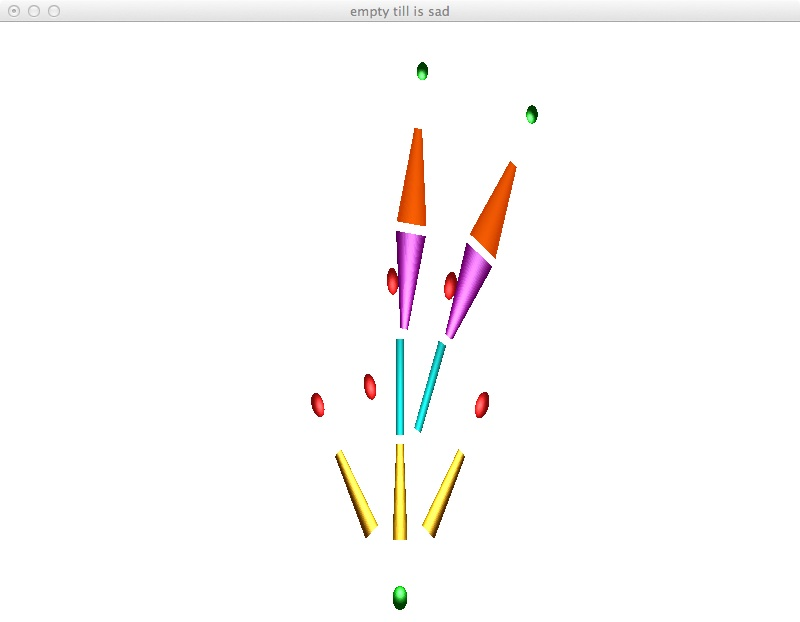
\includegraphics[width=150mm]{emptyTillIsSad.jpg}
\captionfonts
\caption[Oronym Parse Tree]{ This is the parse tree for the phrase ``empty till is sad" }
\label{fig:treeEmptyTillIsSad}
\end{figure}

\begin{figure}
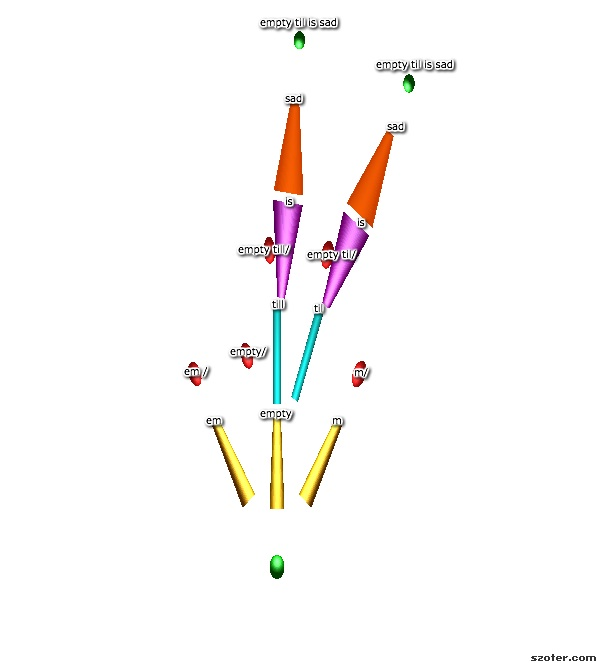
\includegraphics[width=150mm]{emptyTillIsSadAnnotated.jpg}
\captionfonts
\caption[Annotated Oronym Parse Tree]{ This is the annotated parse tree for the phrase ``empty till is sad" }
\label{fig:treeEmptyTillIsSadAnnotated}
\end{figure}



